\chapter{Metodi}
Questo capitolo tratterà le tecnologie, gli strumenti, le librerie e gli algoritmi utilizzati per la realizzazione dei modelli predittivi e dell’interfaccia successivamente creata. 
\section{Tecnologie utilizzate}
\subsection{Machine Learning}

Il Machine Learning, o apprendimento automatico, è un campo di studio che si occupa di sviluppare algoritmi in grado di perfezionarsi automaticamente mediante l'esperienza acquisita tramite l'utilizzo dei dati. 
Gli algoritmi di Machine Learning creano modelli matematici a partire da dati di esempio chiamati "dati di training", in modo da poter attuare predizioni o prendere decisioni senza essere esplicitamente programmati per farlo. 
Esistono tre categorie di approcci di Machine Learning: l'apprendimento supervisionato, l'apprendimento non supervisionato e l'apprendimento per rinforzo.
\begin{itemize}
    \item L'apprendimento supervisionato consiste nell’indicare al calcolatore una regola generale che mappi gli input e gli output desiderati. 
    L'algoritmo di apprendimento è provvisto di dati di input di esempio e degli output corrispondenti e, attraverso successive iterazioni, viene successivamente costruito un modello matematico che può essere sfruttato per predire l'output associato ad un nuovo input.
    \item L'apprendimento non supervisionato invece, non fornisce all'algoritmo di apprendimento le etichette desiderate. 
    In questo caso, l'algoritmo di apprendimento deve necessariamente estrapolare le informazioni significative dai dati di input pur non essendo a conoscenza dell'output desiderato.
    \item L'apprendimento per rinforzo prevede che un programma interagisca con un ambiente dinamico con lo scopo di raggiungere un obiettivo specifico, ad esempio guidare un veicolo o vincere un gioco contro un avversario. 
\end{itemize}
Durante le varie iterazioni il programma riceve un feedback sotto forma di premio e cerca di massimizzare il suo “punteggio”, in modo da imparare e raggiungere l'obiettivo prefissato.

\subsection{Computer Vision}
La Computer Vision è un campo interdisciplinare che si occupa della capacità dei computer di acquisire conoscenza da immagini o video, cercando di replicare il complesso meccanismo alla base dell'apparato visivo umano. 
Questa utilizza metodi per l'acquisizione e l'analisi di immagini digitali in modo da estrarre dati multidimensionali dal mondo reale e produrre informazioni numeriche o simboliche. 
Si avvale pertanto anche di conoscenze di geometria, fisica, statistica e della teoria dell'apprendimento per descrivere il mondo in modo sensato, producendo risultati che possono indirizzarci alla corretta linea d'azione.

\subsection{Cuda}
[da https://developer.nvidia.com/cuda-zone]
CUDA® è una piattaforma di calcolo parallelo, un modello di programmazione sviluppato da NVIDIA per il calcolo generale su unità di elaborazione grafica (GPU). 
Per mezzo di CUDA, gli sviluppatori possono ampliare significativamente la velocità delle applicazioni di calcolo sfruttando la potenza delle GPU.
Nelle applicazioni dotate di accelerazione GPU, la parte sequenziale del carico di lavoro viene eseguita sulla CPU, ottimizzata per le prestazioni single-threaded, mentre la parte computazionalmente intensiva dell’applicazione viene realizzata su migliaia di core GPU in parallelo. 
Quando ci si avvale di CUDA, gli sviluppatori hanno la possibilità di programmare in linguaggi popolari come C, C++, Fortran, Python e MATLAB, esprimendo il parallelismo attraverso estensioni sotto forma di poche parole chiave di base.
Il toolkit CUDA di NVIDIA fornisce tutto il necessario per sviluppare applicazioni con accelerazione GPU.
Il toolkit CUDA include librerie accelerate su GPU, un compilatore, strumenti di sviluppo e il runtime CUDA.

\begin{figure}
    \begin{center}    
        
\includegraphics[width=0.34\linewidth]{images/image1.png}
    \end{center}
\end{figure}

\section{Strumenti utilizzati}
\subsection{Visual Studio Code}
Visual Studio Code è un editor di testo sviluppato da Microsoft per Windows, Linux e macOS, che supporta il debugging, il controllo Git integrato, la Syntax Highlighting, l'IntelliSense, lo Snippet e il refactoring del codice. 
Visual Studio Code supporta molteplici linguaggi e funzionalità aggiuntive grazie alla possibilità di installare dei plugin disponibili attraverso un repository centrale che presenta, oltre a diverse estensioni fornite direttamente da Microsoft, innumerevoli estensioni rese disponibili dalla community. 
\begin{figure}[h]
  \begin{minipage}[b]{0.45\linewidth}
    \centering
    
\includegraphics[width=\linewidth]{images/image2.png}
  \end{minipage}
  \begin{minipage}[b]{0.45\linewidth}
    \centering
    
\includegraphics[width=\linewidth]{images/image3.png}
  \end{minipage}
\end{figure}

\section{Librerie utilizzate}
\subsection{Pandas}
La libreria software open source Pandas è stata sviluppata per il linguaggio di programmazione Python, ed è utilizzata per la manipolazione e l'analisi dei dati. Con Pandas è possibile effettuare operazioni su tabelle numeriche e serie temporali mediante le sue strutture dati. 
Il termine"Pandas" deriva dal termine econometrico "Panel Data", appellativo attribuito a un insieme di dati contenenti osservazioni sugli stessi individui durante più periodi di tempo.
\begin{figure}
    \begin{center}    
        
\includegraphics[width=0.9\linewidth]{images/image4.jpeg}
    \end{center}
\end{figure}

\subsection{Tqdm}
[da https://tqdm.github.io/]
La libreria Python tqdm è uno strumento molto utile per la visualizzazione di barre di avanzamento durante i cicli di elaborazione nel codice. 
Il nome "tqdm" deriva dall'unione della parola araba "taqaddum" che significa "progresso" ed è l'abbreviazione di "te quiero demasiado" (ti amo troppo) in spagnolo. 
Per servirsi della libreria basta inserire qualsiasi iterabile (liste, dizionari, tuple e set) nel metodo della libreria, in questo modo \mintinline[bgcolor=bg]{python}{tqdm(iterable)}. 
La libreria funziona su qualsiasi piattaforma ed è completamente indipendente dalle dipendenze. 
Durante l'estrazione delle Action Units la libreria tqdm ha fornito una stima precisa del tempo necessario per completare l'elaborazione, consentendo di monitorare l'avanzamento del processo in tempo reale. 
Nonostante l'utilizzo della tecnologia CUDA per accelerare le analisi, la grande quantità di immagini da elaborare ha richiesto molto tempo. 
La presenza di tqdm è stata quindi di fondamentale importanza, in quanto ha permesso di gestire efficacemente l'elaborazione dei dati, evitando eventuali problemi tecnici, garantendo risultati accurati ed affidabili e portandomi a riconsiderare delle scelte algoritmiche, non efficientissime, prese. 
In sintesi, la libreria Python tqdm è uno strumento prezioso per semplificare l'elaborazione di grandi quantità di dati, fornendo una stima del tempo rimanente e consentendo di pianificare il lavoro in modo efficiente.

\begin{figure}
    \begin{center}    
        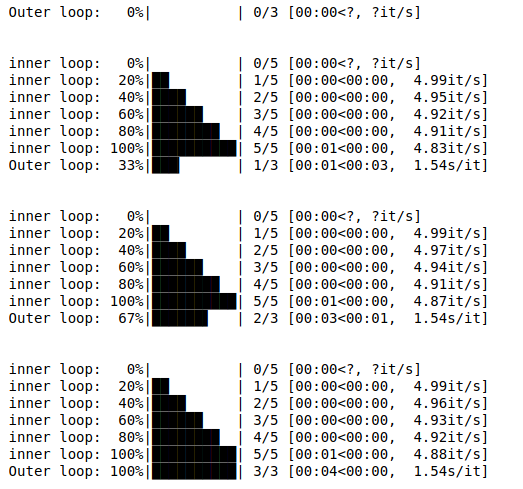
\includegraphics[width=0.9\linewidth]{images/image5.png}
    \end{center}
\end{figure}

\subsection{Pickle}
La libreria pickle è molto versatile e può essere utilizzata per salvare e ripristinare qualsiasi tipo di oggetto Python, inclusi dizionari, liste, tuple, classi e istanze di oggetti personalizzati. 
Inoltre, pickle supporta anche la serializzazione di oggetti multipli in un unico file, rendendo più semplice l'organizzazione dei dati. 
La libreria offre anche diverse opzioni per controllare il comportamento della serializzazione, come la scelta del protocollo di serializzazione e la possibilità di escludere alcuni attributi dall'oggetto da serializzare.
Una caratteristica importante della libreria pickle è che gli oggetti serializzati possono essere utilizzati su diverse piattaforme e versioni di Python, purché il protocollo di serializzazione utilizzato sia compatibile. 
Ciò significa che un oggetto serializzato su un computer Windows con Python 3.9 può essere deserializzato su un computer Linux con Python 2.7, ad esempio. 
Tuttavia, è importante notare che non tutti gli oggetti possono essere serializzati correttamente, come ad esempio le funzioni e le istanze di oggetti di alcune librerie Python. 
Inoltre, la compatibilità tra diverse versioni di Python non è garantita in tutti i casi; quindi, è necessario prestare attenzione a eventuali incompatibilità.

\begin{figure}
    \begin{center}    
        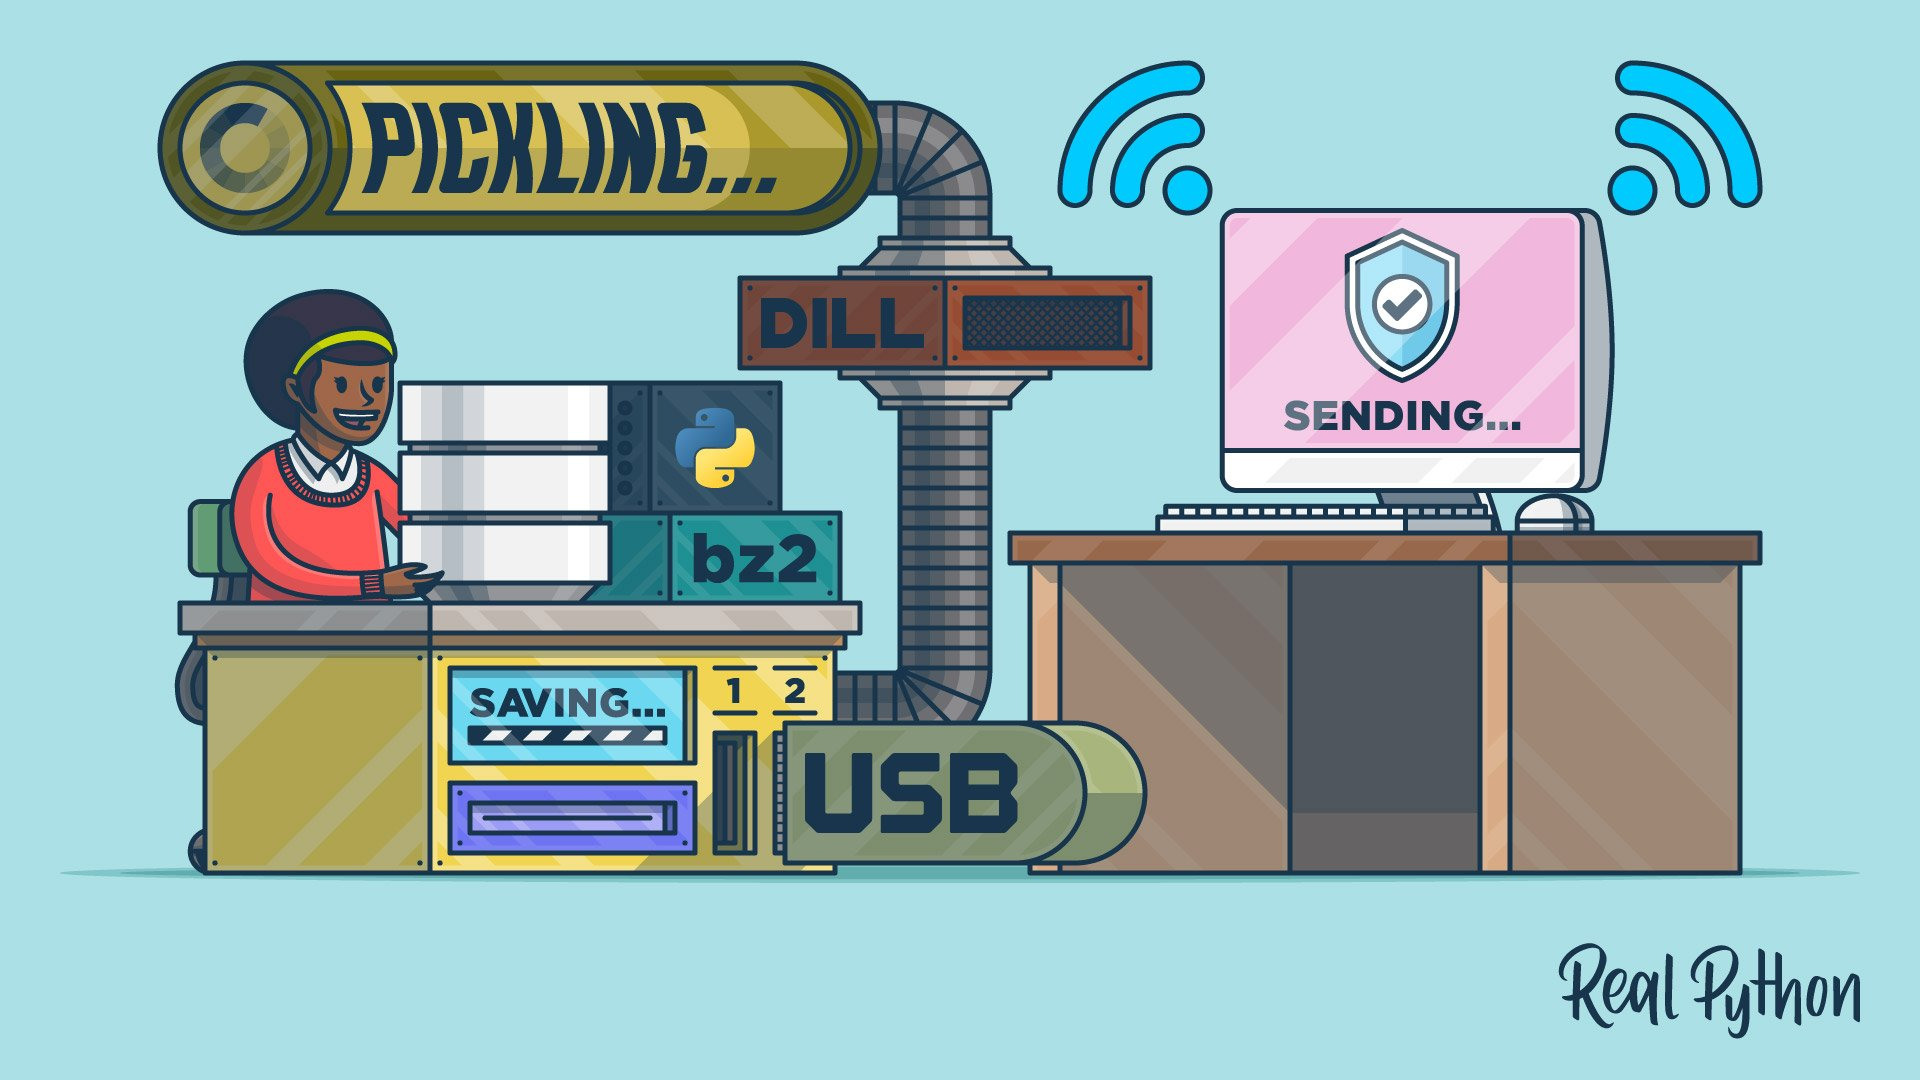
\includegraphics[width=0.9\linewidth]{images/image6.jpeg}
    \end{center}
\end{figure}

\subsection{Torch}
PyTorch è un popolare framework open-source di deep learning che consente agli sviluppatori di creare modelli di intelligenza artificiale in modo rapido ed efficiente. È stato sviluppato originariamente da Facebook AI Research, guadagnandosi una grande popolarità per la sua facilità d'utilizzo, la sua flessibilità e la sua scalabilità.
Una delle sue principali caratteristiche è la sua architettura a flusso di dati (data flow), la quale rende il framework particolarmente adatto per le applicazioni di deep learning. 
Inoltre, PyTorch è dotato di un'ampia gamma di librerie e strumenti come PyTorch Lightning, che mirano a semplificare lo sviluppo di modelli di intelligenza artificiale.
Questa libreria è anche conosciuta per la sua flessibilità e scalabilità, in quanto permette di creare modelli di deep learning sia per computer singoli che per cluster di computer. 
In aggiunta, supporta una vasta gamma di piattaforme hardware, come CPU, GPU e TPU, il che la rende adatta per le applicazioni in ambiti come il machine learning, la visione artificiale e il linguaggio naturale.

\begin{figure}
    \begin{center}    
        
\includegraphics[width=0.9\linewidth]{images/image7.png}
    \end{center}
\end{figure}

\subsection{OpenCV}
[Da https://opencv.org/about/]
OpenCV (Open Source Computer Vision Library) è una libreria software open source finalizzata all’ambito della computer vision e del machine learning. 
È stata ideata per fornire un'infrastruttura comune per le applicazioni di computer vision e per accelerare l'uso della percezione automatica nei prodotti commerciali. 
In quanto prodotto con licenza Apache 2, OpenCV facilita l'utilizzo e la modifica del codice da parte delle aziende.
La libreria contiene più di 2500 algoritmi ottimizzati, che includono un insieme completo di algoritmi di computer vision e machine learning sia classici che all'avanguardia. 
Questi algoritmi possono essere utilizzati per:

\begin{itemize}
  \item rilevare e riconoscere volti, 
  \item identificare oggetti, 
  \item classificare azioni umane nei video, 
  \item tracciare il movimento della telecamera, 
  \item tracciare oggetti in movimento, 
  \item estrarre modelli 3D di oggetti, 
  \item produrre cluster di punti 3D da telecamere stereo, 
  \item unire immagini per produrre un'immagine ad alta risoluzione di un'intera scena, 
  \item trovare immagini simili da un database di immagini, 
  \item rimuovere gli occhi rossi dalle immagini scattate con il flash, 
  \item seguire i movimenti degli occhi, 
  \item riconoscere paesaggi,
  \item creare marker per sovrapporli alla realtà aumentata, ecc. 
\end{itemize}

OpenCV ha più di 47mila utenti nella sua comunità e un numero stimato di download superiore a 18 milioni.
Oltre alle aziende ben consolidate come Google, Yahoo, Microsoft, Intel, IBM, Sony, Honda e Toyota, esistono molte startup come Applied Minds, VideoSurf e Zeitera che ne fanno un uso intensivo. 
Esso è impiegato per molteplici applicazioni, tra cui unire immagini di Street View, rilevare intrusioni in video di sorveglianza in Israele, monitorare l'equipaggiamento minerario in Cina, aiutare i robot a navigare e raccogliere oggetti presso Willow Garage, rilevare gli incidenti di annegamento in piscina in Europa, eseguire arte interattiva in Spagna e New York, controllare le piste di atterraggio per rilevare detriti in Turchia, ispezionare le etichette sui prodotti nelle fabbriche di tutto il mondo e per la rapida rilevazione dei volti in Giappone.
È provvisto di interfacce per C++, Python, Java e MATLAB e supporta Windows, Linux, Android e Mac OS. 
Attualmente sono in sviluppo interfacce complete per CUDA e OpenCL. 
Ci sono oltre 500 algoritmi e circa 10 volte tante funzioni che compongono o supportano questi ultimi.
OpenCV è scritto nativamente in C++ e ha un'interfaccia template che funziona perfettamente con i contenitori STL.

\begin{figure}
    \begin{center}    
        
\includegraphics[width=0.5\linewidth]{images/image8.png}
    \end{center}
\end{figure}

\subsection{Scikit-learn}
[da https://en.wikipedia.org/wiki/Scikit-learn]
Scikit-learn (precedentemente conosciuto come scikits.learn e anche noto come sklearn) è una libreria di machine learning gratuita per il linguaggio di programmazione Python. 
Essa include vari algoritmi di classificazione, regressione e clustering, tra cui support-vector machine, random forest, gradient boosting, k-means e DBSCAN, ed è progettata per funzionare in combinazione con le librerie numeriche e scientifiche di Python, come NumPy e SciPy. 
Il progetto scikit-learn è nato come progetto Google Summer of Code dal data scientist francese David Cournapeau, originariamente chiamato scikits.learn. Il nome del progetto deriva dal concetto di "SciKit" (SciPy Toolkit), un'estensione di terze parti separata e distribuita per SciPy. 
Il codice originale è stato successivamente riscritto da altri sviluppatori. Nel 2010, i contribuenti Fabian Pedregosa, Gaël Varoquaux, Alexandre Gramfort e Vincent Michel dall'Istituto francese per la ricerca in informatica e automazione a Saclay, hanno preso il comando del progetto rilasciando in  seguito la prima versione pubblica della libreria il 1 febbraio 2010. Nel novembre 2012, scikit-learn e scikit-image sono stati descritti come due delle "scikits library" meglio conservate e popolari. 
Nel 2019 si è poi stimato che scikit-learn fosse una delle librerie di machine learning più popolari su GitHub.
Scikit-learn è principalmente scritto in Python e utilizza ampiamente NumPy per l'algebra lineare ad alta prestazione e le operazioni sugli array. 
Inoltre, alcuni algoritmi core sono scritti in Cython per migliorare le prestazioni. Support vector machine è implementato da un wrapper Cython intorno a LIBSVM; la regressione logistica e le macchine a vettori di supporto lineari da un wrapper simile intorno a LIBLINEAR. In tali casi, estendere questi metodi con Python potrebbe non essere possibile.
Scikit-learn si integra bene con molte altre librerie di Python come Matplotlib e Plotly per la visualizzazione dei dati, NumPy per la vettorizzazione degli array, Pandas dataframes, SciPy e molte altre.

\begin{figure}
    \begin{center}    
        
\includegraphics[width=0.7 \linewidth]{images/image9.png}
    \end{center}
\end{figure}

\section{Algoritmi utilizzati per la creazione dei modelli predittivi}
\subsection{Random forest}
Da [https://www.ibm.com/topics/random-forest#:~:text=Random%20forest%20is%20a%20commonly,both%20classification%20and%20regression%20problems.]

\begin{figure}
    \begin{center}    
        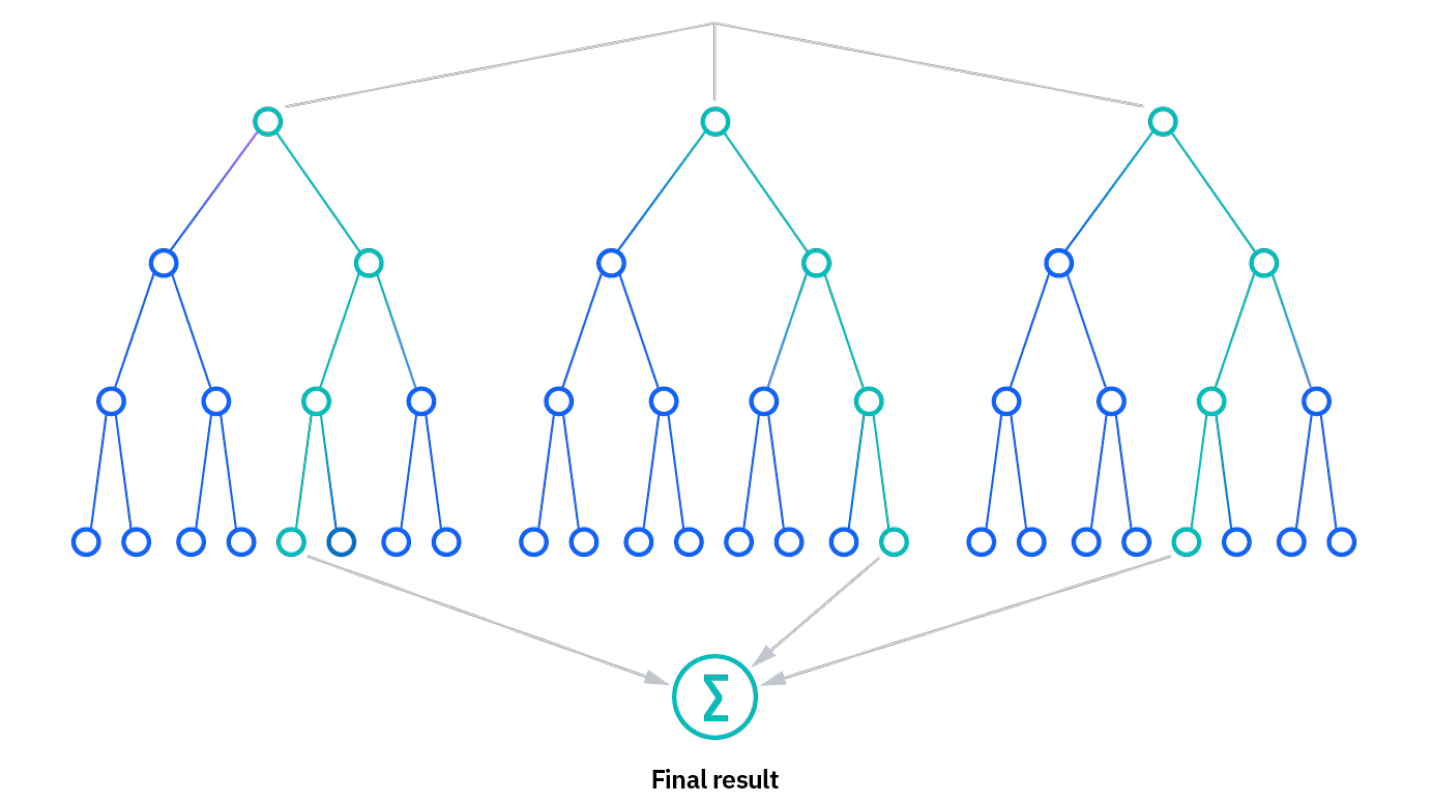
\includegraphics[width=0.9\linewidth]{images/image10.png}
    \end{center}
\end{figure}

La random forest è un algoritmo di apprendimento automatico creato da Leo Breiman e Adele Cutler, che combina l'output di più alberi decisionali col fine di raggiungere un singolo risultato. 
La sua predisposizione intuitiva e la sua flessibilità hanno nutrito l’aumento della sua adozione, in quanto gestisce sia problemi di classificazione che di regressione.

\subsubsection{Alberi decisionali}
Dato che il modello di random forest è composto da più alberi decisionali, è utile descrivere brevemente l'algoritmo dell'albero decisionale. 
Gli alberi decisionali partono da una domanda di base, ad esempio "Dovrei fare surf?". 
A partire da ciò è possibile porre una serie di domande per determinare una risposta, come "C'è un'onda di lungo periodo?" o "Il vento soffia a riva?". 
Queste domande costituiscono i nodi decisionali dell'albero, agendo come mezzo di ripartizione dei dati.
Ogni domanda aiuta l’albero a giungere a una decisione finale, indicata dal nodo foglia raggiunto. 
Le osservazioni che soddisfano i criteri seguiranno il ramo "Sì", mentre quelle che non li soddisfano seguiranno il percorso alternativo. 
Gli alberi decisionali cercano di trovare la miglior suddivisione per i dati, e vengono tipicamente addestrati attraverso l'algoritmo Classification and Regression Tree (CART). 
Metriche come l'impurità di Gini, il guadagno di informazione o l'errore quadratico medio (MSE) possono essere utilizzati per valutare la qualità della suddivisione.
Sebbene gli alberi decisionali siano comuni algoritmi di apprendimento supervisionato, possono essere soggetti a problemi come il bias e l'overfitting. 
Tuttavia, quando più alberi decisionali formano un insieme nell'algoritmo di random forest, predicono risultati più accurati, in particolar modo quando i singoli alberi non sono correlati tra loro.

\subsubsection{L'algoritmo della random forest}
L'algoritmo della random forest è un'estensione del metodo di bagging, in quanto utilizza sia il bagging che la casualità delle features per creare una foresta di alberi decisionali non correlati. 
La casualità delle features, altrimenti nota come bagging delle caratteristiche o "metodo del sottospazio casuale", genera un sottoinsieme casuale di caratteristiche che assicura una bassa correlazione tra gli alberi decisionali. 
Questa è una differenza chiave tra gli alberi decisionali e le random forest, poiché mentre gli alberi decisionali considerano tutte le possibili suddivisioni delle caratteristiche, le random forest selezionano solo un sottoinsieme di quelle caratteristiche.
Tornando all'esempio "dovrei fare surf?", le domande che potrei porre per determinare la previsione potrebbero non essere così esaustive come il set di domande di un altro utente. 
Tenendo conto di tutta la potenziale variabilità dei dati, possiamo ridurre il rischio di overfitting, di bias e di varianza complessiva, ottenendo previsioni via via più precise.

\subsubsection{Come funziona}
Gli algoritmi delle random forest hanno tre iperparametri principali da impostare prima dell'allenamento. 
Questi includono: 

\begin{itemize}
  \item la dimensione del nodo, 
  \item il numero di alberi, 
  \item il numero di caratteristiche campionate
\end{itemize}

Da lì, il classificatore della random forest può essere utilizzato per risolvere problemi di regressione o di classificazione.
L'algoritmo della random forest è costituito da una collezione di alberi decisionali, dove ogni albero nell'insieme è costituito da un campione di dati tratto da un set di allenamento con sostituzione, chiamato campione di bootstrap. 
Di quel campione di allenamento, ad esempio, un terzo viene messo da parte come dati di test, noti come campione fuori dalla borsa (oob), su cui ci soffermeremo in seguito. 
Un'altra istanza di casualità viene quindi iniettata attraverso il bagging delle caratteristiche, incrementando la diversità nel dataset e riducendo la correlazione tra gli alberi decisionali. 
A seconda del tipo di problema, la determinazione della previsione subirà variazioni; per un compito di regressione gli alberi decisionali individuali verranno mediati, mentre per un compito di classificazione una maggioranza di voti, ossia la variabile categorica più frequente, darà come risultato la classe prevista. 
Infine, il campione oob viene utilizzato per la convalida incrociata, finalizzando quella previsione.

\subsubsection{Benefici e sfide del random forest}
Ci sono diversi vantaggi e sfide che l'algoritmo random forest presenta quando utilizzato per problemi di classificazione o regressione. Alcuni di essi includono:

\begin{itemize}
  \item Principali vantaggi
  \begin{itemize}
    \item Riduzione del rischio di overfitting: gli alberi di decisione corrono il rischio di overfitting poiché tendono ad adattarsi strettamente a tutti i campioni all'interno dei dati di formazione. 
    Tuttavia, quando è presente un largo numero di alberi di decisione in un random forest, il classificatore non sovrastimerà il modello, poiché la media di alberi non correlati fra loro riduce la variazione complessiva e l'errore di previsione.
    \item Flessibilità: il random forest può gestire sia compiti di regressione che di classificazione con un elevato grado di precisione, distinguendosi in quanto metodo popolare tra i data scientist. 
    Inoltre, la feature bagging rende il classificatore random forest uno strumento adeguato per la stima dei valori mancanti, in quanto mantiene l'accuratezza quando una parte dei dati è irreperibile.
    \item Facile determinazione dell'importanza delle feature: il random forest rende facile valutare l'importanza delle variabili, o del contributo, al modello. 
    Sussistono alcuni modi per valutare l'importanza della feature; l’importanza di Gini e la diminuzione media dell'impurità (MDI) vengono solitamente utilizzati per misurare quanto diminuisce l'accuratezza del modello quando una determinata variabile viene esclusa.
  \end{itemize}
  \item Principali sfide
  \begin{itemize}
    \item È un processo che richiede tempo: gli algoritmi random forest possono gestire grandi set di dati e fornire previsioni più accurate; tuttavia il processo è rallentato dalla computazione dei dati per ogni singolo albero decisionale.
    \item Richiede più risorse: le random forest, elaborando set di dati più grandi, richiedono più risorse per archiviare questi ultimi.
    \item Più complesso: la previsione di un singolo albero decisionale è più facile da interpretare rispetto a una foresta di questi.
  \end{itemize}
\end{itemize}


\subsection{K-nearest neighbors}
[da https://www.ibm.com/it-it/topics/knn]

\begin{figure}
    \begin{center}    
        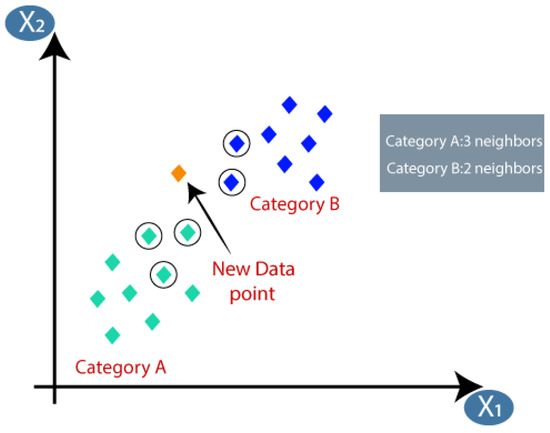
\includegraphics[width=0.9\linewidth]{images/image11.jpeg}
    \end{center}
\end{figure}

L'algoritmo k-nearest neighbors, noto anche come KNN o k-NN, è un classificatore di apprendimento supervisionato non parametrico.
Esso sfrutta la prossimità per effettuare classificazioni o previsioni sul raggruppamento di un singolo punto dati. 
Sebbene possa essere utilizzato per problemi di regressione o classificazione, viene generalmente impiegato in quanto algoritmo di classificazione, basandosi sul presupposto che dati simili, se analizzati o rappresentati nella giusta maniera, possono essere trovati l'uno vicino all'altro.
Per i problemi di classificazione un'etichetta di classe viene assegnata sulla base di un voto a maggioranza(ad es. viene utilizzata l'etichetta più frequentemente rappresentata attorno a un determinato punto dati).
I problemi di regressione utilizzano un concetto simile al problema di classificazione; in questo caso però viene presa la media dei k elementi vicini più vicini per effettuare una previsione su una classificazione. 
Qui, ciò che si discosta notevolmente, è il fatto che la classificazione viene utilizzata per i valori discreti, mentre la regressione viene utilizzata per quelli continui. 
Tuttavia, prima di poter effettuare una classificazione, è necessario definire il concetto di distanza. 
La distanza euclidea, altra metrica di distanza popolare, misura il valore assoluto tra due punti.
Vale la pena notare che l'algoritmo KNN fa anche parte di una famiglia di modelli di "apprendimento pigro", il che significa che memorizza solo un set di dati di addestramento nella fase di addestramento. 
Perviene quindi che tutto il calcolo avvenga quando si compie una classificazione o una previsione. 
Poiché fa ampiamente affidamento sulla memoria per archiviare tutti i suoi dati di addestramento, viene anche definito metodo di apprendimento basato su istanze o basato sulla memoria.
Le idee iniziali sul modello KNN sono attribuite a Evelyn Fix e Joseph Hodges in questo articolo [TODO trova articolo] del 1951, mentre Thomas Cover ne amplia il concetto nella sua ricerca, “Nearest Neighbor Pattern Classification.” [TODO trova articolo] 
Pur non riscuotendo un tale successo come in precedenza, è ancora uno dei primi algoritmi che si affronta nello studio della data science per la sua semplicità ed accuratezza. 
Tuttavia, al crescere di un set di dati KNN diventa sempre più inefficiente, compromettendo le prestazioni del modello. 
Viene riscontrato il suo impiego per semplici sistemi di raccomandazione, riconoscimento di modelli, data mining, previsioni dei mercati finanziari, rilevamento delle intrusioni e altro ancora. 

\subsubsection{Calcolare il KNN: metriche di distanza}
Ricapitolando, l'obiettivo dell'algoritmo k-nearest neighbor è identificare i vicini più prossimi di un dato punto di query, in modo da poter assegnare un'etichetta di classe a quel punto. 
Per determinare quali punti dati sono più attigui ad un determinato punto di query, sarà necessario calcolare la distanza tra il punto di interrogazione e gli altri punti dati. 
Le metriche di distanza aiutano a formare confini decisionali che suddividono i punti di query in regioni diverse. 
Sebbene sussistano diverse misure di distanza, tra cui è possibile scegliere, l’articolo sul sito di IBM tratta esclusivamente quelle a seguire:
\begin{itemize}
    \item Distanza euclidea (p=2): la misura della distanza più comunemente adottata; essa è limitata ai vettori con valori reali. 
    Utilizzando la formula seguente traccia una linea retta tra il punto di query e l'altro punto che si vuole misurare.
    \begin{figure}
        \begin{center}    
            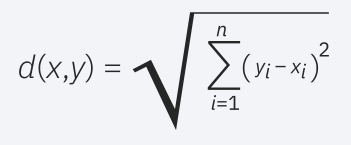
\includegraphics[width=0.45\linewidth]{images/image12.png}
        \end{center}
    \end{figure}
    \item Distanza di Manhattan (p=1): un'altra metrica di distanza particolarmente nota che si propone di misurare il valore assoluto tra due punti. 
    È anche riconosciuta come distanza del taxi o distanza del blocco cittadino, poiché è comunemente visualizzata con una griglia che illustra come si potrebbe percorrere il tragitto da un indirizzo all'altro attraverso le strade della città.
    \begin{figure}
        \begin{center}    
            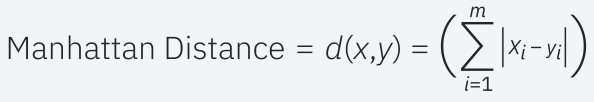
\includegraphics[width=0.45\linewidth]{images/image13.png}
        \end{center}
    \end{figure}
    \item Distanza di Minkowski: questa misura della distanza è la forma generalizzata delle metriche di distanza euclidea e di Manhattan. Il parametro, p, nella formula seguente, consente la creazione di altre metriche di distanza.    
    La distanza Euclidea è rappresentata da questa formula quando p è uguale a due e la distanza di Manhattan è indicata con p uguale a uno.

    \begin{figure}
        \begin{center}    
            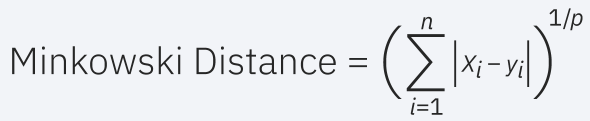
\includegraphics[width=0.45\linewidth]{images/image14.png}
        \end{center}
    \end{figure}

    \item Distanza di Hamming: questa tecnica viene utilizzata tipicamente con vettori booleani o stringa, identificando i punti in cui i vettori non trovano corrispondenza. 
    Di conseguenza, è stata anche definita metrica di sovrapposizione.
    \begin{figure}
        \begin{center}    
            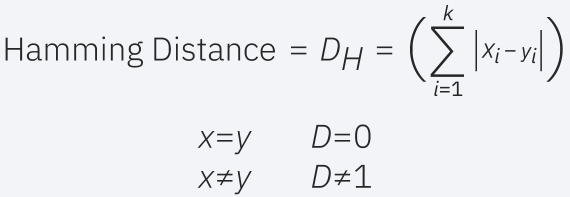
\includegraphics[width=0.45\linewidth]{images/image15.png}
        \end{center}
    \end{figure}
\end{itemize}

\newpage
Ad esempio, se avessi le seguenti stringhe, la distanza di Hamming sarebbe due poiché solo due dei valori differiscono.

\begin{figure}
    \begin{center}    
        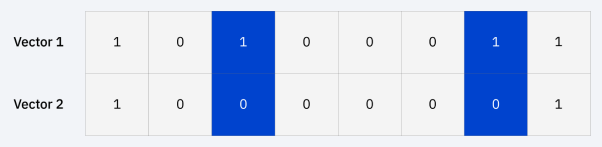
\includegraphics[width=0.8\linewidth]{images/image16.png}
    \end{center}
\end{figure}

\subsubsection{Calcolare KNN: definizione di k}
Il valore k nell'algoritmo k-NN definisce quanti vicini verranno controllati per determinare la classificazione di un punto di query specifico. 
Di fatti, se k=1, l'istanza verrà assegnata alla stessa classe del suo singolo neighbors più vicino. 
Definire k può essere un atto di bilanciamento, in quanto valori diversi possono portare a overfitting o underfitting. 
Valori inferiori a k possono essere caratterizzati da una variabilità elevata ma una bassa distorsione, mentre valori maggiori di k possono portare a una distorsione elevata e una variabilità inferiore. 
La scelta di k dipenderà in particolar modo dai dati di input, dal momento che i dati con più valori anomali o rumore probabilmente opereranno in modo più proficuo tanto più elevati sono i valori di k. 
In generale si consiglia di adoperare un numero dispari per k, col fine di evitare pareggi nella classificazione.

\subsubsection{Applicazioni di k-NN nell'apprendimento automatico}
L'algoritmo k-NN è stato utilizzato all'interno di una varietà di applicazioni, in maggior misura all'interno della classificazione. Alcuni di questi casi d'uso includono:
\begin{itemize}
\item Pre-elaborazione dei dati: poichè i dataset presentano spesso valori mancanti, l'algoritmo KNN può stimare tali valori in un processo noto come imputazione dei dati mancanti.
\item Recommender systems: adoperando i dati del flusso di clic dai siti web, l'algoritmo KNN è stato utilizzato per fornire consigli automatici agli utenti su contenuti aggiuntivi. Da tale ricerca emerge che un utente è assegnato a un particolare gruppo e, sulla base del comportamento di quest'ultimo, riceve un consiglio. Tuttavia, dati i problemi di scalabilità con KNN, questo approccio potrebbe non risultare ottimale in caso di impiego di dataset più grandi.
\item Finanza: è stato utilizzato anche in una varietà di casi di utilizzo finanziari ed economici. Ipoteticamente, un articolo mostra in che modo l'utilizzo di KNN sui dati di credito può aiutare le banche nella valutazione dei rischi su un prestito a un'organizzazione o a un individuo. Viene quindi sfruttato per determinare l'affidabilità creditizia del richiedente di tale prestito. Un altro articolo ne sottolinea l'uso nelle previsioni del mercato azionario, nei tassi di cambio, nel trading di fetures e nelle analisi sul riciclaggio di denaro.
\item Assistenza sanitaria: KNN ha riscontrato applicazioni anche nel settore dell'assistenza sanitaria, effettuando previsioni sul rischio di infarto e cancro alla prostata. L'algoritmo funziona calcolando le espressioni geniche più probabili.
\item Riconoscimento dei pattern: KNN ha anche aiutato a identificare i pattern, come nel testo e nella classificazione digitale. Ciò è stato particolarmente utile per identificare i numeri scritti a mano in cui ci si potrebbe imbattere su moduli o buste postali.
\end{itemize}
\subsubsection{Vantaggi e svantaggi dell'algoritmo KNN}
K-NN possiede i suoi punti di forza e di debolezza. A seconda del progetto e dell'applicazione, potrebbe rivelarsi o meno la scelta giusta.
\begin{itemize}
\item Vantaggi
\begin{itemize}
\item Facile da implementare: data la semplicità e l'accuratezza dell'algoritmo, è uno dei primi classificatori che un data scientist alle prime armi apprenderà.
\item Si adatta facilmente all'aggiunta di nuovi campioni di addestramento, l'algoritmo si adatta per tenere conto di eventuali nuovi dati, a fronte dell'archivio di tutti i dati di addestramento in memoria.
\item Pochi iperparametri: KNN necessita solo di un valore k e una metrica di distanza, il che, a confronto con altri algoritmi di machine learning, è minore in quantità.
\end{itemize}
\item Svantaggi
\begin{itemize}
\item Non è provvisto di una buona scalabilità: essendo KNN un algoritmo cosiddetto pigro, occupa più memoria e spazio di storage dei dati rispetto ad altri classificatori.
Sebbene diverse strutture di dati ,come Ball-Tree, siano state create per affrontare le inefficienze computazionali, un classificatore diverso potrebbe dimostrarsi ideale.
\item Maledizione della dimensionalità: l'algoritmo tende a cadere vittima della “maledizione della dimensionalità”; ciò significa che non ricopre adeguatamente il proprio ruolo con input di dati ad alta dimensionalità.
Questo è a volte indicato anche come il fenomeno del picco, nel quale, dopo che l'algoritmo raggiunge l'ottimale numero di funzioni, le funzioni aggiuntive aumentano la quantità di errori di classificazione, soprattutto quando la dimensione del campione è inferiore.
\item Propensione al sovradimensionamento dei dati: a causa della "maledizione della dimensionalità", KNN è anche più propenso al sovradimensionamento dei dati.
Sebbene le tecniche di selezione delle caratteristiche e di riduzione della dimensionalità vengano sfruttate per evitare che ciò accada, il valore di k può inevitabilmente influire sul comportamento del modello.
Valori più bassi di k possono sovra-alimentare i dati, mentre valori più alti di k tendono a "smussare" i valori di previsione, poiché si sta attuando la media dei valori su un'area o un neighborhood più grande.
Tuttavia, se il valore di k è troppo alto, può essere inferiore ai dati.
\end{itemize}
\end{itemize}

\subsection{Naive Bayes Classifier}
[da https://towardsdatascience.com/naive-bayes-classifier-81d512f50a7c]
Un classificatore di Bayes è un modello di apprendimento automatico probabilistico utilizzato per compiti di classificazione. Il fulcro del classificatore si basa sul teorema di Bayes.


\subsubsection{Teorema di Bayes}
Utilizzando il teorema di Bayes, possiamo trovare la probabilità che A accada, conseguentemente all’avvenimento di B. Qui, B è la prova e A è l'ipotesi. 
L'assunzione alla base del teorema è che i predittori e le caratteristiche siano indipendenti: in altre parole, la presenza di una particolare caratteristica non influisce sull'altra.
\begin{figure}
    \begin{center}    
        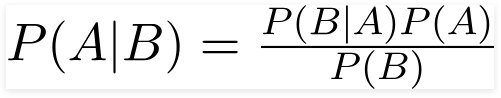
\includegraphics[width=0.9\linewidth]{images/image17.png}
    \end{center}
\end{figure}
Volendo offrire un esempio al fine di una migliore comprensione, consideriamo il problema di giocare a golf.  Il dataset è rappresentato come segue.
\begin{figure}
    \begin{center}    
        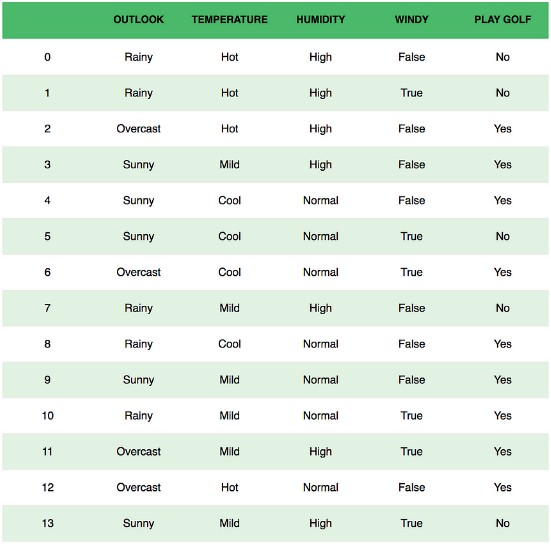
\includegraphics[width=0.9\linewidth]{images/image18.jpeg}
    \end{center}
\end{figure}
Classifichiamo se la giornata si configura adatta per una partita di golf, basandoci sugli attributi di tale giornata. Le colonne rappresentano questi attributi, mentre le righe rappresentano le singole voci.
Prendendo a campione la prima riga del dataset, possiamo osservare che non è adatta per giocare a golf se il cielo è nuvoloso, la temperatura è calda, l'umidità è alta e non c'è vento. Qui facciamo due assunzioni: 
come già detto, consideriamo che questi predittori siano indipendenti (ovvero, se la temperatura è calda, non significa necessariamente che l'umidità sia alta). Un'altra assunzione fatta qui è che tutti i predittori abbiano un effetto uguale sul risultato. Cioè, il fatto che ci sia vento non ha una maggiore importanza nella  decisione di giocare a golf o meno. 


Rifacendosi al secondo esempio, il teorema di Bayes può essere quindi riscritto come segue:

\begin{figure}
    \begin{center}    
        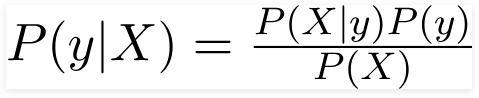
\includegraphics[width=0.9\linewidth]{images/image19.png}
    \end{center}
\end{figure}
La variabile y è la variabile di classe (giocare a golf), la quale rappresenta quanto sia adatta la giornata o meno per giocare a golf. La variabile X rappresenta i parametri/caratteristiche.


X è dato come segue:
\begin{figure}
    \begin{center}    
        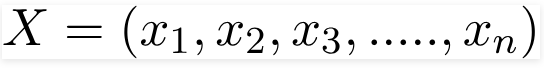
\includegraphics[width=0.9\linewidth]{images/image20.png}
    \end{center}
\end{figure}
Qui x1, x2... xn raffigurano le caratteristiche, cioè possono essere mappati su cielo, temperatura, umidità e vento. Sostituendo X ed espandendo utilizzando la regola della catena otteniamo:
\begin{figure}
    \begin{center}    
        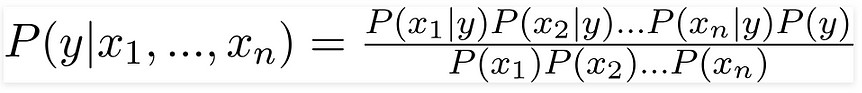
\includegraphics[width=0.9\linewidth]{images/image21.jpeg}
    \end{center}
\end{figure}
Ora è possibile ottenere i valori per ognuno guardando il dataset e sostituendoli nell'equazione. Per tutte le voci nel dataset, il denominatore non cambia, rimane statico. Pertanto, il denominatore può essere rimosso e può essere introdotta una proporzionalità.

\begin{figure}
    \begin{center}    
        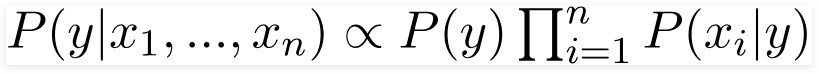
\includegraphics[width=0.9\linewidth]{images/image22.jpeg}
    \end{center}
\end{figure}
Nel nostro caso, la variabile di classe (y) ha solo due risultati, sì o no. Potrebbero esserci casi in cui la classificazione potrebbe rivelarsi multivariata. Pertanto, sarà necessario trovare la classe y con la massima probabilità.

\begin{figure}
    \begin{center}    
        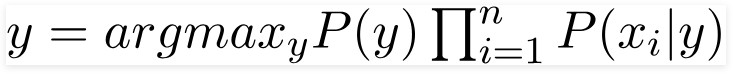
\includegraphics[width=0.9\linewidth]{images/image23.jpeg}
    \end{center}
\end{figure}
Utilizzando questa funzione ci è possibile ottenere la classe, dato il predittore.




\subsubsection{Tipi di Classificatori Bayesiani}
\begin{itemize}
\item Classificatore Bayesiano Multinomiale:
\begin{itemize}
\item Esso è principalmente utilizzato per problemi di classificazione dei documenti; ad esempio, se un documento appartiene alla categoria di sport, politica, tecnologia, ecc. Le caratteristiche/predittori impiegati dal classificatore saranno la frequenza delle parole presenti nel documento.
\end{itemize}
\item Classificatore Bayesiano di Bernoulli:
\begin{itemize}
\item Questo classificatore è simile al precedentemente citato, pur essendo i predittori variabili booleane. I parametri che usiamo per prevedere la variabile di classe assumono solo valori sì o no (se una parola compare nel testo o meno).
\end{itemize}
\item Classificatore Bayesiano Gaussiano:
\begin{itemize}
\item Quando i predittori assumono un valore continuo e non discreto, assumiamo che questi valori siano estratti da una distribuzione gaussiana.
\end{itemize}
\end{itemize}
Poiché il modo in cui i valori sono presenti nel dataset cambia, la formula per la probabilità condizionata cambia in questo caso,
\begin{figure}
    \begin{center}    
        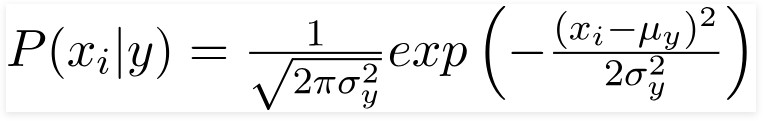
\includegraphics[width=0.9\linewidth]{images/image24.jpeg}
    \end{center}
\end{figure}

\subsubsection{Conclusione}
 
Gli algoritmi Bayesiani sono principalmente utilizzati nell'analisi del sentiment, nel filtraggio dello spam, nei reccomender systems, ecc. 
Sono veloci e facili da implementare, ma il loro più grande svantaggio è la necessità che i predittori siano indipendenti. 
Nella maggior parte dei casi reali, i predittori sono dipendenti, il che ostacola le prestazioni del classificatore.




\subsection{Support Vector Machine}
Il support vector machine è favorito maggiormente data la produzione di una significativa accuratezza mediante una minor potenza di calcolo. 
Il Support Vector Machine, abbreviato come SVM, può essere utilizzato sia per compiti di regressione che di classificazione. Tuttavia, viene ampiamente sfruttato negli obiettivi di classificazione.
\subsubsection{Cosa è il Support Vector Machine?}
L'obiettivo dell'algoritmo support vector machine è quello di trovare un iperpiano in uno spazio N- dimensionale (N - il numero di caratteristiche) che classifichi distintamente i punti dati.
\begin{figure}[h]
  \begin{minipage}[b]{0.45\linewidth}
    \centering
    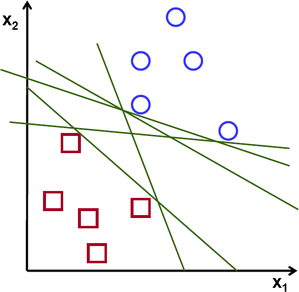
\includegraphics[width=\linewidth]{images/image25.png}
  \end{minipage}
  \begin{minipage}[b]{0.45\linewidth}
    \centering
    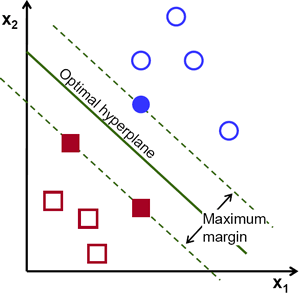
\includegraphics[width=\linewidth]{images/image26.png}
  \end{minipage}
\end{figure}
Per separare le due classi di punti dati sono presenti molti iperpiani possibili da cui poter scegliere. Il nostro obiettivo è trovare un piano che possegga il margine massimo, ovvero la massima distanza tra i punti dati di entrambe le classi. Massimizzare la distanza del margine fornisce un rinforzo in modo che i futuri punti dati possano essere classificati con maggiore fiducia.
Iperpiani e support vector

\begin{figure}
    \begin{center}    
        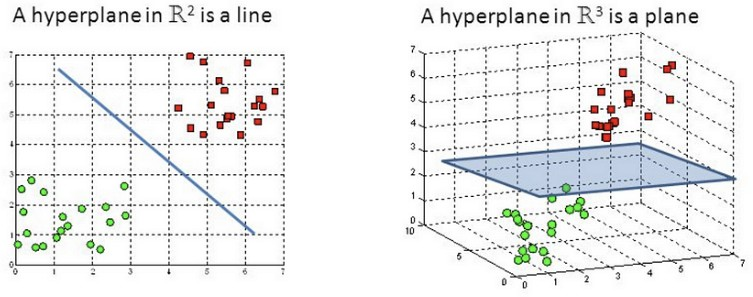
\includegraphics[width=0.9\linewidth]{images/image27.jpeg}
    \end{center}
\end{figure}
Gli iperpiani sono i confini decisionali che aiutano a classificare i punti dati. 
I punti dati che cadono su entrambi i lati dell'iperpiano possono essere attribuiti a diverse classi. 
Inoltre, la dimensione dell’iperpiano  dipende dal numero di caratteristiche. 
Se il numero di caratteristiche di input è 2, l'iperpiano è solo una linea. Se il numero di caratteristiche di input è 3, l'iperpiano diventa un piano bidimensionale. Diventa difficile immaginare quando il numero di caratteristiche supera 3.

\begin{figure}
    \begin{center}    
        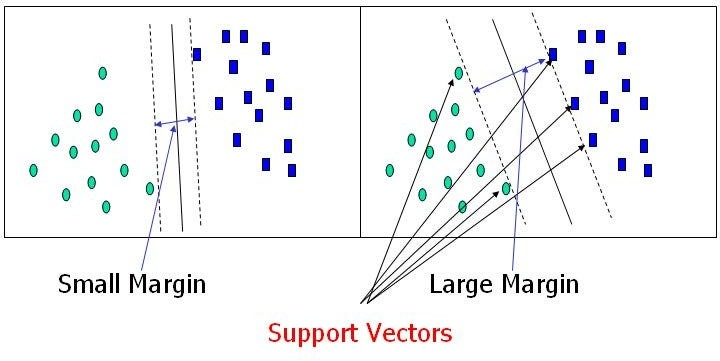
\includegraphics[width=0.9\linewidth]{images/image28.jpeg}
    \end{center}
\end{figure}
I support vector sono i punti dati più vicini all'iperpiano e influenzano la posizione e l'orientamento di quest’ultimo. Impiegando i support vector, massimizziamo il margine del classificatore. L’eliminazione  dei support vector cambierà la posizione dell'iperpiano. 


\subsubsection{Intuizione del grande margine}
Nella regressione logistica, prendiamo l'output della funzione lineare e normalizziamo il valore nell'intervallo  [0,1] utilizzando la funzione sigmoide. 
Se il valore normalizzato è maggiore di un valore soglia (0,5), gli assegniamo una etichetta 1, altrimenti gli assegniamo un'etichetta 0. 
Nell'SVM, prendiamo l'output della funzione lineare e, se quell'output è maggiore di 1, lo identifichiamo con una classe, mentre se l'output è -1, lo identifichiamo con un'altra classe. 
Poiché i valori della soglia sono cambiati in 1 e -1 nell'SVM, otteniamo questo intervallo ([-1,1]) che viene utilizzato come margine.


\subsubsection{Funzione di costo e aggiornamenti del gradiente}
Nell'algoritmo SVM, cerchiamo di massimizzare la distanza tra i punti dati e l'iperpiano. La funzione di perdita che ci aiuta a massimizzare la distanza è la hinge loss.
\begin{figure}[h]
  \begin{minipage}[b]{0.45\linewidth}
    \centering
    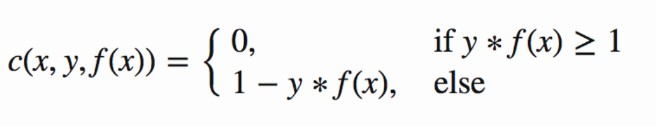
\includegraphics[width=\linewidth]{images/image29.jpeg}
  \end{minipage}
  \begin{minipage}[b]{0.45\linewidth}
    \centering
    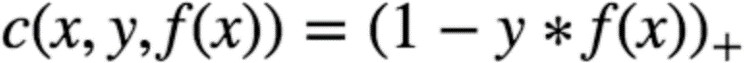
\includegraphics[width=\linewidth]{images/image30.jpeg}
  \end{minipage}
\end{figure}

Il costo è 0 se il valore previsto e il valore effettivo hanno lo stesso segno. In caso contrario, calcoliamo il valore di perdita. Aggiungiamo anche un parametro di regolarizzazione alla funzione di costo. L'obiettivo del
 
parametro di regolarizzazione è di bilanciare la massimizzazione della distanza con la perdita. 
Dopo aver aggiunto il parametro di regolarizzazione, la funzione di costo appare come segue.
\begin{figure}
    \begin{center}    
        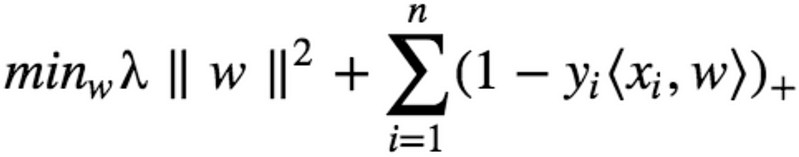
\includegraphics[width=0.9\linewidth]{images/image31.jpeg}
    \end{center}
\end{figure}
Ora che abbiamo ottenuto la funzione di perdita, utilizziamo le derivate parziali rispetto ai pesi per trovare i gradienti. 
Così facendo, possiamo aggiornare i pesi.
\begin{figure}
    \begin{center}    
        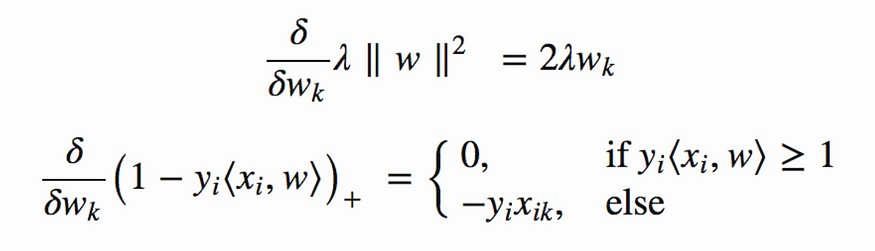
\includegraphics[width=0.9\linewidth]{images/image32.jpeg}
    \end{center}
\end{figure}
Quando non vi è alcuna errata classificazione, ovvero il nostro modello prevede correttamente la classe del nostro punto dati, sarà necessario aggiornare solo il gradiente dal parametro di regolarizzazione.
\begin{figure}
    \begin{center}    
        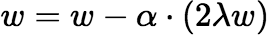
\includegraphics[width=0.9\linewidth]{images/image33.png}
    \end{center}
\end{figure}
Quando ci si trova di fronte ad una errata classificazione, ossia il nostro modello commette un errore sulla previsione della classe del nostro punto dati, includiamo la perdita insieme al parametro di regolarizzazione per eseguire l'aggiornamento del gradiente.


\begin{figure}
    \begin{center}    
        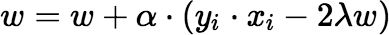
\includegraphics[width=0.9\linewidth]{images/image34.png}
    \end{center}
\end{figure}